\documentclass[italian]{beamer}

\hypersetup{unicode=true,
	%bookmarks=true,
	bookmarksnumbered=false,
	bookmarksopen=false,
	breaklinks=false,
	pdfborder={0 0 0},
	%backref=false,
	colorlinks=false,
	pdfpagemode=FullScreen,
	pdfauthor={Gionata Massi},
	pdfsubject={Presentazione della prova orale del concorso docenti 2016, classe di concorso A41 Scienze e tecnologie informatiche, di Gionata Massi.},
	pdfkeywords={Concorso docenti, A41, Informatica.}%
}

\usepackage[T1]{fontenc}
\usepackage[latin1]{inputenc}
\usepackage{babel}
%\usepackage{pgfpages}
%\usepackage{standalone}
\usepackage{verse}
\usepackage{booktabs}
\usepackage{multirow}
\usepackage{bookmark}
\usepackage{graphicx}
%\usepackage{eurosym}
%\usepackage{pgfplots}
%\usepgfplotslibrary{dateplot}     
\usepackage{tikz}
\usetikzlibrary{shapes}
\newcommand*\circled[1]{\tikz[baseline=(char.base)]{%
		\node[shape=ellipse,draw,inner sep=2pt] (char) {#1};}}

%\usepackage[]{algorithm2e}
%\usepackage{xmpmulti}

\usepackage{calc}
\usepackage[font=Times,timeinterval=59, timeduration=45.0, timedeath=1, fillcolorwarningsecond=white!60!yellow,
timewarningfirst=78,timewarningsecond=95]{tdclock}


\pgfdeclareimage[height=5mm]{CONCORSO}{img/banner_concorso_docenti}
\logo{\pgfuseimage{CONCORSO}}

\newcommand{\blu}[1]{{\usebeamercolor[fg]{structure} #1}}
\newcommand{\red}[1]{{\usebeamercolor[fg]{alerted text} #1}}



\setbeamertemplate{navigation symbols}{}
%\setbeamertemplate{frametitle continuation}[from second][(cont'd)]
\usefonttheme[stillsansseriftext,stillsansserifsmall]{serif}

\makeatletter

\mode<beamer|trans>{%
	\useoutertheme[glossy]{wuerzburg}
	\useinnertheme[shadow,outline]{chamfered}
	\usecolortheme{shark}
}


%% Save up on ink for the 4-up handouts
\mode<handout>{%
	\useoutertheme{wuerzburg}
	\useinnertheme[outline]{chamfered}
	%\pgfpagesuselayout{4 on 1}[a4paper, landscape, border shrink=10mm]
	\pgfpagesuselayout{2 on 1}[a4paper, portrait, border shrink=10mm]
	\pgfpageslogicalpageoptions{1}{border code=\pgfstroke}
	\pgfpageslogicalpageoptions{2}{border code=\pgfstroke}
	%\pgfpageslogicalpageoptions{3}{border code=\pgfstroke}
	%\pgfpageslogicalpageoptions{4}{border code=\pgfstroke}
}

\mode<presentation>{%
	\AtBeginSection{%
		\begin{frame}
			\frametitle{In questa sezione\ldots}
			\tableofcontents[ %
			currentsection,%
			hideothersubsections,%
			sectionstyle=show/hide,% 
			subsectionstyle=show/hide%
			]
		\end{frame}
	}
}		
		
\title[Concorso docenti CdC A41]
{\Large{Processo di risoluzione degli indirizzi a livello applicativo}}

\institute[I.T.A. ``E. Sereni'']
{%
	{\scriptsize
Concorso personale docente\\
DD.DD.GG. n. 105, 106 e 107 del 23 febbraio 2016\\
Classe di concorso A41 -- Scienze e tecnologie informatiche}
}

\date[Roma, 21/07/2016 {\usebeamercolor[fg]{frametitle}\textbar}~\cronominutes]{Roma -- 21 Luglio 2016}

\newcommand\mybullet{\leavevmode%
\blu{\usebeamertemplate{itemize item}}\hspace{.5em}}

\begin{document}

\author[G. Massi]{%
	Ing. \textit{Gionata \textsc{Massi}}, PhD
}

\frame{\maketitle\initclock}
% \beamerdefaultoverlayspecification{<+->}
% \setbeamercovered{dynamic}

%\section*{Piano della presentazione}
%\subsection{Parte I: Esposizione di un percorso didattico}
\newcommand\boxednumber[1]
{%
	\hbox{%
		\usebeamerfont*{item projected}%
		\usebeamercolor[bg]{item projected}%
		\vrule width2.25ex height1.85ex depth.4ex%
		\hskip-2.25ex%
		\hbox to2.25ex{%
			\hfil%
			\color{fg}#1%
			\hfil}%
	}%
}

\begin{frame}{Piano della presentazione}
	\boxednumber{1} Parte~~~I: Illustrazione delle scelte contenutistiche, didattiche e metodologiche
	
	\medskip
	
	\boxednumber{2} Parte~~II: Esposizione di una lezione simulata
	
	\medskip
	\boxednumber{3} Parte~III: Interlocuzioni con il candidato
	\note{%
		{\tiny
			Buon pomeriggio,
			
			sono Gionata Massi e presenter\`o un percorso didattico sulla traccia estratta, riassunta dal titolo \dots.
			In 35 minuti dovrei illustrarvi la progettazione del percorso didattico, ipotizzando
			di avere di fronte una classe tipo e risorse didattiche infinite.
			
		}%tiny
	}%note
\end{frame}

\frame{
	\frametitle{Piano della presentazione del percorso didattico}
	\tableofcontents[part=1]
	\note{%
		{\tiny
			Buon pomeriggio,
			
			sono Gionata Massi e presenter\`o un percorso didattico sul \dots.
			
		}%tiny
	}%note
}

\frame{
	\frametitle{Piano della lezione}
	\tableofcontents[part=2]
	}

\frame{
	\frametitle{Piano del colloquio}
	\begin{center}\Huge{Any questions?}\end{center}
	}

\part[Percorso didattico]{Esposizione di un percorso didattico}
\frame{\partpage}

\section[Contesto]{Il contesto - traccia e ipotesi}

\begin{frame}{Traccia estratta}{Estratto}

	\begin{block}{\ldots{}il candidato analizzi il seguente caso concreto:}
		\large{processo di risoluzione degli indirizzi a livello applicativo}
	\end{block}
	
	\begin{block}{Su cosa devo preparare una lezione?}
		\begin{itemize}
			\item Lezione partecipata sul \alert<2>{Domain Name System (DNS)} con IPv4.
			\item Attivit\`a di aboratorio usando \texttt{nslookup} e \texttt{wireshark}.
			\item Con pi\`u di 24 avrei potuto progettare il laboratorio sull'analisi dei file \texttt{/etc/hosts} e \texttt{/etc/resolv.conf} e per la configurazione di \texttt{bind} su una rete di calcolatori emulata.
		\end{itemize}
	\end{block}

\end{frame}

\begin{frame}{Scelta dell'istituto, della classe e della disciplina}{ITT -- I\&T -- Informatica -- classe $4^{\text{ta}}$ -- Sistemi e reti}
	
	\begin{block}{Istituto, settore, indirizzo, articolazione, disciplina}
		\noindent\mybullet Istituto \alert{Tecnico}
		
		\noindent\hspace*{0.5cm}\mybullet Settore \alert{Tecnologico} (Economico)
		
		\noindent\hspace*{1.0cm}\mybullet Indirizzo ``\alert{Informatica e Telecomunicazioni}''  (Amministrazione, Finanza e Marketing)
		
		\noindent\hspace*{1.5cm}\mybullet Articolazione ``\alert{Informatica}'' (Sistemi Informativi Aziendali)
		
		\noindent\hspace*{2.0cm}\mybullet \alert{Sistemi e reti} (Informatica)
	\end{block}
	
	\begin{block}{Territorio}
	\begin{itemize}
		\item Regione Marche
		\begin{itemize}
			\item PMI, pi\`u piccole che medie
			\item sviluppo di applicazioni gestionali
			\item settore telecomunicazioni e radar
			\item sistemi di misura e controllo
		\end{itemize}	
	\end{itemize}
	\end{block}
\end{frame}
	
\begin{frame}{Ipotesi della classe e situazione iniziale}{ITT -- I\&T -- Informatica -- classe $4^{\text{ta}}$ -- Sistemi e reti}
	
	\begin{block}{Classe}
		\begin{itemize}
			\item Classe $4^{\text{ta}}$
			\begin{itemize}
				\item 132 ore annue $\approx$ 4 ore a settimana
				\item di cui 2 in compresenza con l'insegnante tecnico pratico
				\item stimo circa 2$\frac{1}{2}$ ore settimanali di studio autonomo
			\end{itemize}			
			\item 20 alunni (18M / 2F)
			\item 0 alunni ripetenti
			\item 1 alunno BES disgrafico con PDP
			\item la maggioranza degli alunni con livello medio/alto
			\item gli studenti svolgono lezione in laboratorio, con una postazione PC per ogni alunno
			\item il laboratorio \`e dotato di proiettore e lavagna bianca
		\end{itemize}
	\end{block}
	
\end{frame}

\section[Progettazione didattica]{Progettazione didattica}

\begin{frame}[allowframebreaks]{Quadro normativo}
%{Le leggi, le linee guida, le direttive ministeriali}
{Linee guida e direttive ministeriali}

	\begin{block}{d.P.R. n. 88 del 15 marzo 2010, articolo 8, comma 3 -- All. A.2}
		\noindent {\color{blue!50!black}``ISTITUTI TECNICI -- LINEE GUIDA PER IL PASSAGGIO AL NUOVO ORDINAMENTO''}
		% http://hubmiur.pubblica.istruzione.it/alfresco/d/d/workspace/SpacesStore/fd8ad76e-0e72-4ff2-aeff-0264b98168c3/linee_guida_tec_doc_completo_15_07_2010.pdf#page=63
		\medbreak
		\noindent\textbf{Presentazione sintetica ITT -- I\&T, estratto della pagina 63}
		\medbreak
		\mybullet L'indirizzo ``Informatica e Telecomunicazioni'' integra \alert{competenze} scientifiche e \alert{tecnologiche nel campo} dei sistemi informatici, dell'elaborazione delle informazioni, delle applicazioni e tecnologie Web, \alert{delle reti} e degli apparati \alert{di comunicazione}; \textit{omissis}
	\end{block}
	
	\begin{block}{Direttiva n. 4  del 16 gennaio 2012}
		\noindent {\color{blue!50!black} \textbf{in materia di Linee Guida per il secondo biennio e quinto anno per i percorsi degli Istituti Tecnici a norma dell'articolo 8, comma 3 del d.P.R. del 15 marzo 2010, n. 88.}}
		\medbreak
		Definisce, negli allegati, le schede disciplinari per il secondo biennio e quinto anno.
		\medbreak
		Allegato C4, ``ISTITUTI TECNICI -- LINEE GUIDA PER IL PASSAGGIO AL NUOVO ORDINAMENTO -- Schede disciplinari Secondo biennio e quinto anno''
		%http://banner.orizzontescuola.it/B1_AFM.pdf#page=3
	\end{block}\label{dir:16012012}
\end{frame}

\begin{frame}[allowframebreaks]{Indicazioni ministeriali}{Schede disciplinari -- Indirizzo ``Informatica'' -- ``Sistemi e Reti'', estratti All. C4}
		\begin{tabular}{p{\dimexpr \linewidth-2\tabcolsep}}
		\toprule
		\multicolumn{1}{c}{\bf Risultati di apprendimento del secondo biennio e quinto anno}\\
		\midrule
			\mybullet \alert<2>{configurare, installare e gestire sistemi di elaborazione dati e reti}\\
			\mybullet scegliere dispositivi e strumenti in base alle loro caratteristiche funzionali\\
			\mybullet utilizzare le reti e gli strumenti informatici nelle attivit\`a di studio, ricerca e approfondimento disciplinare\\
			\mybullet \alert<2>{analizzare il valore, i limiti e i rischi delle varie soluzioni tecniche} per la vita sociale e culturale con particolare attenzione alla sicurezza nei luoghi di vita e di lavoro, alla tutela della persona, dell'ambiente e del territorio\\
		\bottomrule
		\end{tabular}
		
		\centering
		\begin{tabular}{p{0.49\dimexpr \linewidth-2\tabcolsep}p{0.49\dimexpr \linewidth-2\tabcolsep}}
		\toprule
		\multicolumn{2}{c}{\bf Secondo biennio}\\
		\multicolumn{1}{c}{\bf Conoscenze} & \multicolumn{1}{c}{\bf Abilit\`a}\\
		\midrule
			\mybullet \alert<4>{Organizzazione del software di rete in livelli} & \mybullet Individuare la corretta \alert<4>{configurazione di una data applicazione}\\
			\mybullet Tipologie  e \alert<4>{tecnologie delle reti locali e geografiche} & \mybullet Progettare, realizzare, configurare e gestire una rete\\
			\mybullet \alert<4>{Protocolli per la comunicazione in rete}\\
			\mybullet \alert<4>{Tecniche di gestione dell'indirizzamento di rete}\\
			\mybullet Problematiche di instradamento nelle reti geografiche\\
			\mybullet Lessico e terminologia tecnica di settore anche in lingua inglese & \mybullet Utilizzare il lessico e la terminologia tecnica di settore anche in lingua inglese\\
		\bottomrule
		\end{tabular}
		
	\note{%

	}%note	
\end{frame}

%\begin{frame}{Programmazione didattica}{Quadro normativo delle attivit\`a funzionali all'insegnamento}
%	\begin{block}{CCNL Scuola 2006/2009 art. 29}
		
%		1. L'attivit\`a funzionale all'insegnamento {[}\ldots{]} comprende
%		tutte le attivit\`a, anche a carattere collegiale, di programmazione, progettazione,
%		ricerca, valutazione, documentazione, aggiornamento e formazione {[}\ldots{]}
		
%		\medskip
		
%		2. Tra gli adempimenti individuali dovuti rientrano le attivit\`a relative: 
		
%		\hspace*{0.5cm}a) alla preparazione delle lezioni e delle esercitazioni;
		
%	\end{block}
%\end{frame}

%\begin{frame}[allowframebreaks]{Definizioni}{Quadro europeo delle qualifiche}
%	\begin{description}
%		\item[risultati dell'apprendimento] descrizione di ci\`o
%		che un discente conosce, capisce ed \`e in grado di
%		realizzare al termine di un processo d'apprendimento.
%		I risultati sono definiti in termini di conoscenze,
%		abilit\`a e competenze;
		
%		\item[conoscenze] risultato dell'assimilazione di
%		informazioni attraverso l'apprendimento. Le
%		conoscenze sono un insieme di fatti, principi, teorie
%		e pratiche relative ad un settore di lavoro o di studio.
%		Nel contesto del Quadro europeo delle qualifiche
%		le conoscenze sono descritte come teoriche e/o
%		pratiche;
		
%		\item[abilit\`a] indicano le capacit\`a di applicare
%		conoscenze e di utilizzare know-how per portare a
%		termine compiti e risolvere problemi. Nel contesto
%		del Quadro europeo delle qualifiche le abilit\`a sono
%		descritte come cognitive (comprendenti l'uso del
%		pensiero logico, intuitivo e creativo) o pratiche
%		(comprendenti l'abilit\`a manuale e l'uso di metodi,
%		materiali, strumenti);
		
%		\item[competenze] comprovata capacit\`a di utilizzare
%		conoscenze, abilit\`a e capacit\`a personali, sociali
%		e/o metodologiche, in situazioni di lavoro o di
%		studio e nello sviluppo professionale e personale.
%		Nel contesto del Quadro europeo delle qualifiche
%		le competenze sono descritte in termini di
%		responsabilit\`a e autonomia.
%	\end{description}
%\end{frame}

\begin{frame}{Programmazione didattica}{Chi, come, perch\'e}

\mybullet Visto il P(T)OF, considerato il territorio e le specificit\`a dell'Istituto,
\alert{il Dipartimento d'Informatica} stabilisce una pianificazione di massima identificando, per ogni anno di corso, i moduli didattici.

\mybullet Ogni modulo ha una collocazione temporale e indica i prerequisiti, i risultati d'apprendimento (espressi in termini di competenze, conoscenze e abilit\`a), la durata temporale, i metodi e i materiali didattici e la tipologia e il numero minimo di verifiche, le prove comuni.

\mybullet Il docente pu\`o integrare la programmazione, di concerto con il consiglio di classe, con UdA e compiti autentici, per la certificazione di competenze trasversali.

\mybullet La parte seguente \`e la mia progettazione di un ciclo di lezioni nel modulo sul livello di applicazione, che segue quelli sui livelli di rete e trasporto, limitatamente al ``Domain Name System''.

\end{frame}

\begin{frame}[allowframebreaks]{Prerequisiti, conoscenze pregresse, motivazioni}{Per la programmazione e la riprogettazione dell'attivit\`a didattica}

%	Non si pu\`o programmare un'attivit\`a didattica senza conoscere la classe.
	
%	Andrebbero lette le relazioni finali e verificate le conoscenze in ingresso!
	
	Assumeremo che i seguenti prerequisititi di conoscenza siano stati conseguiti (e certificati).
		
	\begin{block}{Prerequisiti e conoscenze pregresse}
		I concetti base e gli aspetti implementativi dei protocolli delle applicazioni di rete
		
		\begin{itemize}
			\item la commutazione di pacchetto, i protocolli IP e TCP;
			\item i modelli di servizio del livello di trasporto (livello 4 del modello ISO/OSI);
			\item i modelli di servizio del livello di rete (livello 3 del modello ISO/OSI);
			\item il paradigma client-server;
			\item la composizione di una URL.
		\end{itemize}
	\end{block}
	
	%\begin{block}{Conoscenze pregresse che l'insegnante pu\`o sondare}
	%	Gli studenti hanno gi\`a esperienza d'uso del Web e di altre applicazioni di rete realizzate con le tecnologie del Web.
		
	%	\medskip
		
	%	I ``nativi digitali'' sono stati tenuti all'oscuro di quanto c'\`e dietro ad un software. Questo \`e materia di sondaggio per la progettazione dell'attivit\`a didattica e di motivazione.
	%\end{block}
	
	%\framebreak
	
	%\framebreak

	%\begin{block}{Esperienze pregresse}
	%	Scambiare informazioni/comunicare tra esseri umani
	%	\begin{itemize}
	%		\item \textbf{blog};
	%		\item \textbf{forum}
	%		\item \textbf{social network}
	%		\item \textbf{wiki};
	%		\item \textbf{giochi online}
	%	\end{itemize}
		
	%	Soddisfare esigenze specifiche con web application
	%	\begin{itemize}
	%		\item \textbf{commercio elettronico}
	%		\item \textbf{mappe} e \textbf{ricerca di percorsi} in un grafo stradale
	%		\item \textbf{web-mail}
	%		\item \textbf{calendari} e \textbf{strumenti collaborativi}
	%	\end{itemize}
	%\end{block}
		
	\begin{block}{Motivare allo studio: fare leva sui bisogni di}
		\begin{description}
			\item[autostima] stima da parte dei compagni e degli insegnanti\\\hfill\textbf{peer assessment}
			\item[auto-efficacia] apportare il proprio contributo\\\hfill\textbf{peer assessment, mini-progetto}
			\item[potere] dominare la realt\`a\\\hfill\textbf{(ri)conoscere architetture e tecnologie della rete}
			\item[avere uno scopo] dare un senso alle nozioni apprese\\\hfill\textbf{configurare bind, analizzare con sniffer, riconoscere minacce, mini-progetto}
			\item[sfida] difficolt\`a da superare\\\hfill\textbf{mini-progetto}
		\end{description}
	\end{block}
\end{frame}

\subsection[Finalit\`a]{Obiettivi generali}
\begin{frame}{Obiettivi generali}{Le finalit\`a del modulo didattico}
	Con riferimento alle competenze, alle conoscenze e alle abilit\`a definite dalla Direttiva n. 4 del 16/01/2012 in materie di Linee Guida per la classe prescelta \hyperlink{dir:16012012}{\beamerreturnbutton{estratto linee guida}}, si raffina l'unit\`a didattica sui Linguaggi del Web allo scopo di sviluppare le competenze per:
	
	\begin{itemize}
		\item \alert{progettare, sviluppare e realizzare una ``web page'' moderna
		usando i linguaggi HTML, CSS e JavaScript.}
	\end{itemize}
	
	\begin{exampleblock}{Nota sulla scelta dei linguaggi per il Web}
		Le finalit\`a indicate dal ministero sottointendono la realizzazione di pagine lato client. Non si includono nel percorso del terzo anno quei linguaggi per la realizzazione del back-end (JavaScript/Node.js, Python, PHP, Java\ldots{}), lo scambio dati (es: JSON, XML) o la loro strutturazione e interrogazione (SQL).
	\end{exampleblock}
	\note{%
		
	}%note	
\end{frame}

\subsection[Obiettivi]{Obiettivi d'apprendimento}
\begin{frame}[allowframebreaks]{Obiettivi come prestazioni misurabili}{Concetti del web}
	
	% 		\item Comprendere quali sono i principali componenti architetturali di una ``web page'' moderna e le loro inter-connessioni.
	
	{\tiny
	\begin{table}
		\begin{tabular}{@{}p{0.2\textwidth}p{0.75\textwidth}@{}} \toprule
			\multicolumn{1}{c}{Abilit\`a} & \multicolumn{1}{c}{Obiettivo} \\ \midrule
			
			\multirow{3}{*}{\parbox{0.2\textwidth}{Comprendere ed utilizzare il linguaggio tecnico}}
			 & Elencare le componenti di un'applicazione di rete.\\
			 & Definire i ruoli delle componenti dell'architettura client/server e i flussi di dati ed elaborazioni.\\
			 & Elencare le componenti del servizio World Wide Web (WWW).\\
			 & Elencare i metodi del protocollo HTTP.\\
			 & Elencare le intestazioni pi\`u rilevanti del protocollo HTTP. \\
			 & Mettere in relazione richiese e risposte HTTP.\\
			 & Definire i termini \textit{ipertesto}, \textit{Uniform Resource Locator} (URL), \textit{collegamento ipertestuale} (\textit{hyperlink}), \textit{web hosting}, \textit{motore di ricerca}.\\
			 
			 \\
			 
			 \multirow{3}{*}{\parbox{0.2\textwidth}{Usare il browser per sviluppare contenuti per il web}}
			 & Visualizzare richeste e riposte HTTP intercorse fra il browser e il server Web.\\
			 & Visualizzare le intestazioni HTTP.\\
			 & Visualizzare il codice sorgenti delle risorse scaricate.\\
			 & Accedere alla console JavaScript del browser.\\
			 & Emulare la visualizzazione della pagina su un dispositivo mobile, sapendo scegliere i parametri della rete.\\
			 & Visualizzare la timeline delle richieste e del loro download.\\ \bottomrule
		\end{tabular}
		\caption{Il linguaggio tecnico. Usare il browser}
	\end{table}
	}
	
	\framebreak
	
	{\tiny
		\begin{table}
			\begin{tabular}{@{}p{0.2\textwidth}p{0.75\textwidth}@{}} \toprule
				\multicolumn{1}{c}{Abilit\`a} & \multicolumn{1}{c}{Obiettivo} \\ \midrule
				
				\multirow{3}{*}{\parbox{0.2\textwidth}{Veicolare contenuti sul web}}
				& Identificare i principali vantaggi che l'utilizzo di un	sito web comporta: accesso a un pubblico esteso, facilit\`a di aggiornamento, interattivit\`a con gli utilizzatori e benefici di costi.\\
				
				& Elencare in ordine cronologico le fasi del processo di pubblicazione di un sito web: registrazione del dominio, scelta del servizio di un internet provider.\\
				
				& Usare tecniche che possono migliorare l'efficacia dei motori di ricerca, come: utilizzo di
				metadati indicativi, mappa del sito e collegamenti ipertestuali al sito stesso, registrazione presso un motore di ricerca.\\
				
				& Identificare i fattori che possono impattare sulla rapidit\`a di download di una pagina web: contenuti audio, video, grafici, animazioni, file compressi.\\
				
				& Saper valutare quale formato \`e pi\`u appropriato per i file audio, video, grafici in modo da migliorare la velocit\`a di download delle pagine web.\\
				
				\\
				
				\multirow{3}{*}{\parbox{0.2\textwidth}{Uso di base del linguaggio HTML}}
				& Comprendere il termine HyperText Markup Language (HTML).\\
				& Riconoscere il ruolo e le raccomandazioni del consorzio W3C. Comprendere i vantaggi che si
				possono avere seguendo queste raccomandazioni: interoperabilit\`a dei siti web fra i diversi browser in commercio, miglioramento dell?accessibilit\'a, corretta dichiarazione del tipo di documento (doctype).\\
			\end{tabular}
			\caption{Editoria sul web. Fondamenti di HTML}
		\end{table}
	}
	
	\framebreak
	
	{\tiny
	\begin{table}
		\begin{tabular}{@{}p{0.2\textwidth}p{0.75\textwidth}@{}} \toprule
			\multicolumn{1}{c}{Abilit\`a} & \multicolumn{1}{c}{Obiettivo} \\ \midrule
			
			\multirow{2}{*}{\parbox{0.2\textwidth}{Progettazione}}
			& Riconoscere, programmare ed utilizzare tecniche
			per: valutare le necessit\`a degli utilizzatori, creare
			storyboard, organizzare la struttura del sito, creare
			un modello di pagina del sito, definire uno schema
			di navigazione.\\
			& Riconoscere le parti (sezioni) in cui \`e diviso un sito internet.\\ 
			& Riconoscere i tipi di carattere (font) sui siti web\\
			& Riconoscere i tipi di carattere con grazie, senza grazie, monospaziati.\\
			& Riconoscere gli stili tondo, inclinato, neretto, maiuscoletto.\\
			& Indicare per quale parte di un documento \`e consigliato l'uso di un certo tipo di carattere.\\
			
			\\
			
			\multirow{3}{*}{\parbox{0.2\textwidth}{Collegamenti ipertestuali}}
			
			& Usare il  tag <href> con collegamenti ipertestuale
			assoluti e relativi.\\
			& Inserire un collegamento
			ipertestuale da una parola di testo o da
			un'immagine.\\
			& Inserire un collegamento
			ipertestuale di posta elettronica: da una parola di
			testo o da un'immagine.\\
			& Definire un riferimento per un collegamento, nella
			stessa finestra, in una nuova finestra, in un frame.\\
			& Assegnare un segnalibro (anchor), per creare un
			collegamento all'interno della stessa pagina, inserire
			un collegamento su di un segnalibro.
			\\ \bottomrule
		\end{tabular}
		\caption{Progettazione. Collegamenti ipertestuali}
	\end{table}
	}
	
	{\tiny
		\begin{table}
			\begin{tabular}{@{}p{0.2\textwidth}p{0.75\textwidth}@{}} \toprule
				\multicolumn{1}{c}{Abilit\`a} & \multicolumn{1}{c}{Obiettivo} \\ \midrule
				
				\multirow{3}{*}{\parbox{0.2\textwidth}{Concetti sui fogli
						di stile - CSS}}
				& Comprendere il termine fogli di stile (Cascading
				Style Sheets - CSS), utilizzo e benefici.\\
				& Riconoscere gli approcci principali di applicazione
				degli stili: in linea, interni, esterni.\\ 
				& Comprendere la struttura delle regole di stile:
				selettore, blocco di dichiarazione (propriet\`a e
				valore).\\
				
				\\
				
				\multirow{3}{*}{\parbox{0.2\textwidth}{Utilizzo dei fogli di
						stile}}
				& Creare, salvare un nuovo foglio di stile CSS.\\
				& Creare, modificare le regole di stile: colore, sfondo,
				tipo di carattere.\\
				& Associare un foglio di stile CSS esterno ad una
				pagina web.\\
				
				\\
				
				\multirow{3}{*}{\parbox{0.2\textwidth}{Pubblicazione}}
				& Riconoscere buone pratiche nella realizzazione di
				contenuti web: includere la data dell'ultimo
				aggiornamento, specificare i dettagli del software
				necessario per aprire, visualizzare file, assicurare la
				compatibilit\`a dei contenuti con i principali browser
				web.\\
				& Comprendere il processo di caricamento,
				scaricamento di un sito web, verso o da un server.\\
				& Caricare, scaricare un sito web verso o da un
				server.
				\\ \bottomrule
			\end{tabular}
			\caption{Fogli di stile. Pubblicazione}
		\end{table}
	}
	
\end{frame}

\subsection[Strategie\ldots]{Metodologie, strategie e strumenti didattici utilizzati}

\begin{frame}[fragile]{Un approccio laboratoriale}{Apprendimento guidato dall'esperimento}
	
	\begin{columns}
		\begin{column}{0.3\textwidth}
			
			\newcommand{\autore}[1]{%
				\nopagebreak{\raggedleft\footnotesize #1\par}}
				
			\settowidth{\versewidth}{Se ascolto dimentico,}
			{\color{green!50!black}	
			\begin{verse}[\versewidth]
			\begin{altverse}
				Se ascolto dimentico,\\
				Se vedo ricordo,\\
				Se faccio imparo\\
				\autore{Confucio}
			\end{altverse}
			\end{verse}
			}
			
			\vfill
			
			\begin{itemize}
				\item in laboratorio;
				\item col computer;
				\item tanti elaborati;
				\item peer assessment;
				\item mini-progetto.
			\end{itemize}
			
			Quali fasi?
						
		\end{column}
		
		\begin{column}{0.7\textwidth}
			
			\begin{enumerate}
				\item Elicitazione delle conoscenze pregresse su web e sue tecnologie e motivazione con esempi derivanti esperienze;
				
				\item proposizione di problematiche, esposizione di strategie risolutive, sperimentazione al computer;
				
				\item prove formative in itinere con produzione di elaborati individuali (web page);
				
				\item prova sommativa, illustrazione della soluzione e peer assessment;
				
				\item mini-progetto con potenziamento e/o recupero.
			\end{enumerate}			
			
		\end{column}
	\end{columns}

	\note{%
		
	}%note	
\end{frame}

\subsection[Strumenti\ldots]{Software di ausilio alla didattica}
\begin{frame}{Strumenti per imparare facendo}{Con cosa esercitarsi}
	\begin{itemize}
		\item Chromium
		
		\item Mozilla Firefox
		
		\item La pagina ipertestuale \hyperlink{https://www.khanacademy.org/computer-programming/new/webpage}{https://www.khanacademy.org/computer-programming/new/webpage}.
		
		\item La pagina ipertestuale \hyperlink{http://www.w3schools.com/}{http://www.w3schools.com/}
		
		\item Node.js
	\end{itemize}
	\note{%
		
	}%note	
\end{frame}

\section[Modi e tempi]{Modi e tempi del segmento didattico}
\begin{frame}{Modi e tempi}{Pianificazione delle lezioni}
	
	\begin{itemize}
		\item 36 ore.
		\item 18 ore di lavoro autonomo per studio e valutazione peer-assessment.		
	\end{itemize}
	\medskip
	\medskip
%	\centering\includegraphics[trim={2cm 14.5cm 2cm 2cm},clip,width=0.95\textwidth]{img/gantt}		
\end{frame}


\section[Verifica e valutazione]{Verifica e valutazione}
\begin{frame}{Valutazione condivisa}{Valutazione per spingere al miglioramento}
	
	\begin{itemize}
		\item verifiche formative a casa, una dopo ogni lezione teorica, con quiz a risposta multipla
		\item peer assessment di 3 elaborati prodotti dai compagni di classe (double-blind)
		\item mini-progetto
	\end{itemize}
	
%	\centering\includegraphics[width=0.6\textwidth]{img/mini_progetto}
	\note{%
		
	}%note	
\end{frame}

\section[Adattamenti per BES]{Adattamenti per BES}
\begin{frame}{Strumenti compensativi e misure dispensative}{Per BES e DSA}
	
	Strumenti compensativi
	\begin{itemize}
		\item si usano gi\`a strumenti informatici ``compensativi''
		\item l'argomento non presenta livelli di astrazione elevati
	\end{itemize}
	
	Misure dispensative
	
	\begin{itemize}
		\item a seconda del caso:
		\begin{itemize}
			\item aumento del tempo della prova
			\item dispensa da esercizi pi\`u astratti
			\item programmazione per obiettivi minimi
			\item prove oggettive
			\item dispensa dal valutare altre prove
		\end{itemize}
	\end{itemize}
	
	Recupero individualizzato, in particolare durante le ore in compresenza.
			
	\note{%
		
	}%note	
\end{frame}


\part[Lezione simulata]{Esposizione della lezione}
\frame{\partpage}

\section[nslookup]{Query con \texttt{nslookup}}

\begin{frame}{Interrogare il DNS}{Usare \texttt{nslookup}}

\only<1,3,5,7>{
\begin{block}{Sfide -- usare \texttt{nslookup} in modo interattivo}
\begin{block}{Leggere insieme la pagina di manuale di \texttt{nslookup}}
\texttt{man nslookup}
\end{block}

Chiedere in modo interattivo l'indirizzo dell'host \texttt{ricop.dii.univpm.it}
\begin{enumerate}
	\item al name server predefinito 
	\item \uncover<3->{al name server 8.8.8.8}
	\item \uncover<5->{abilitando la visualizzazione completa del pacchetto di risposta}
	\item \uncover<7->{visualizzando le informazioni sull'host}
\end{enumerate}
\end{block}
}
\only<2>{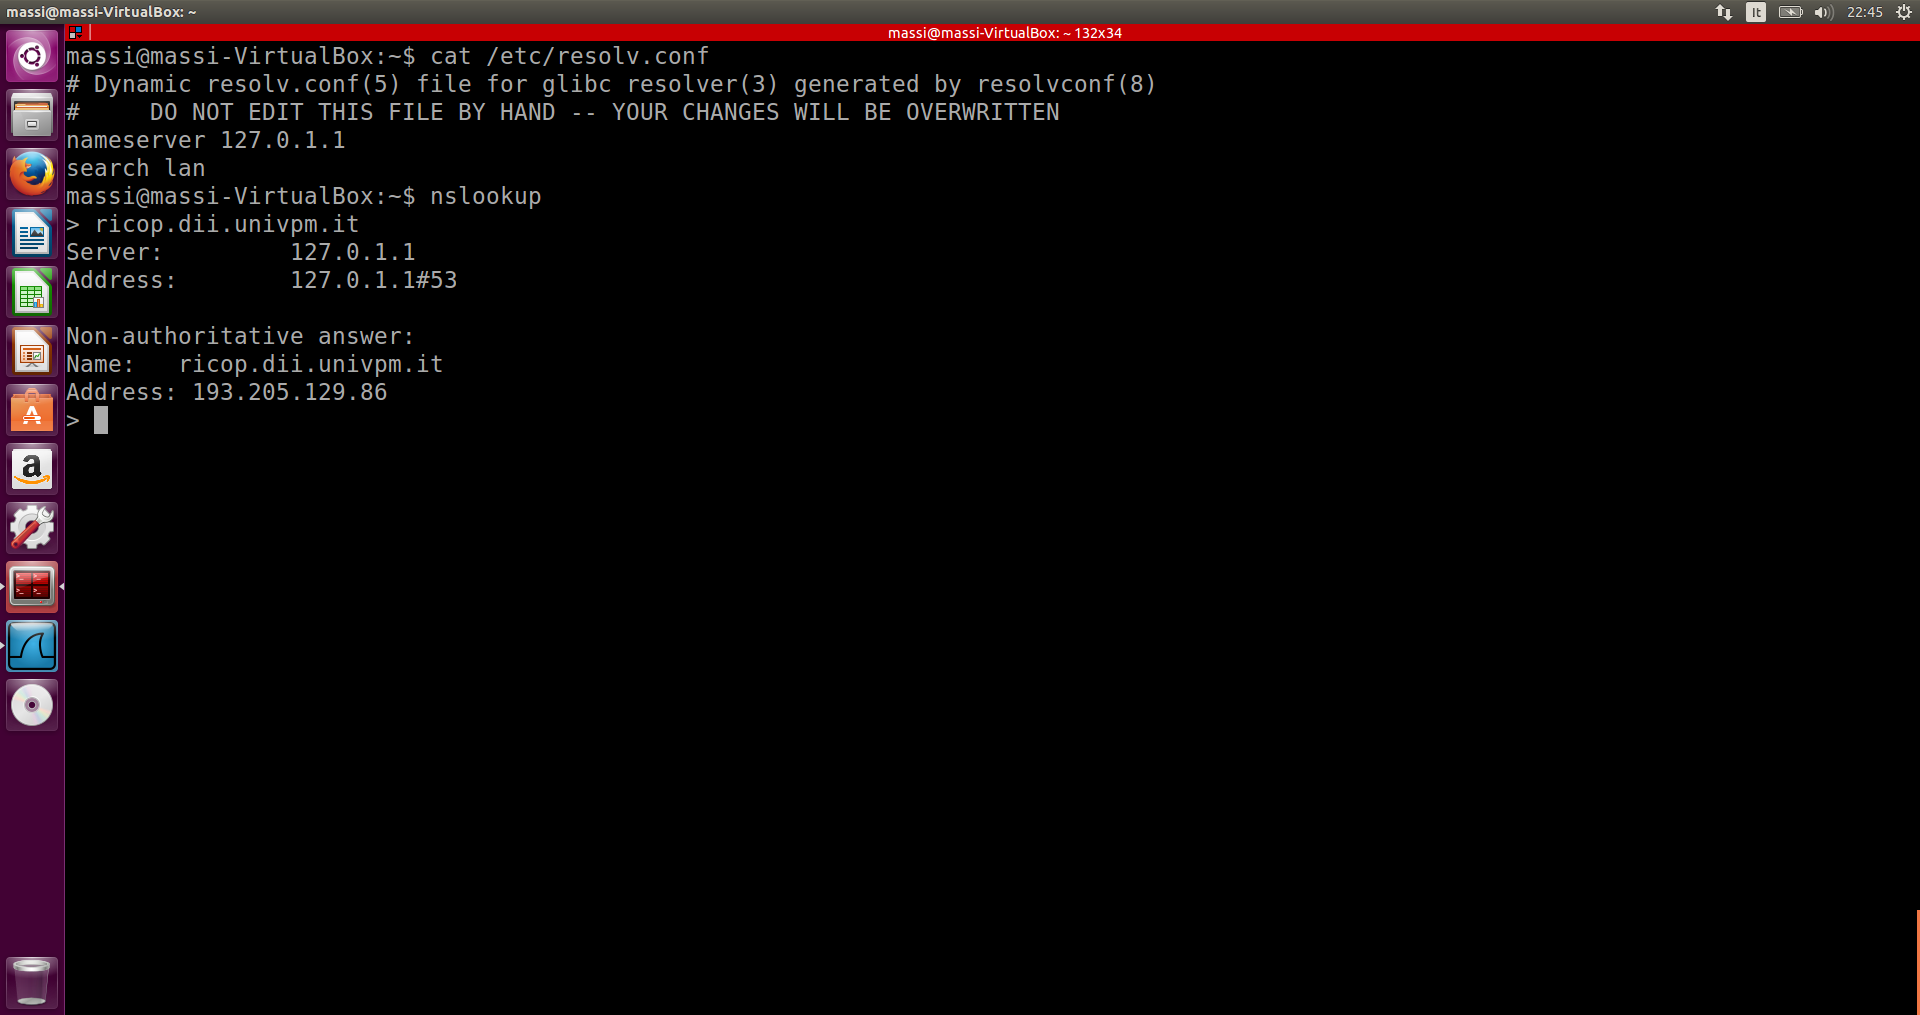
\includegraphics[width=\textwidth]{img/lab1_1}}
\only<4>{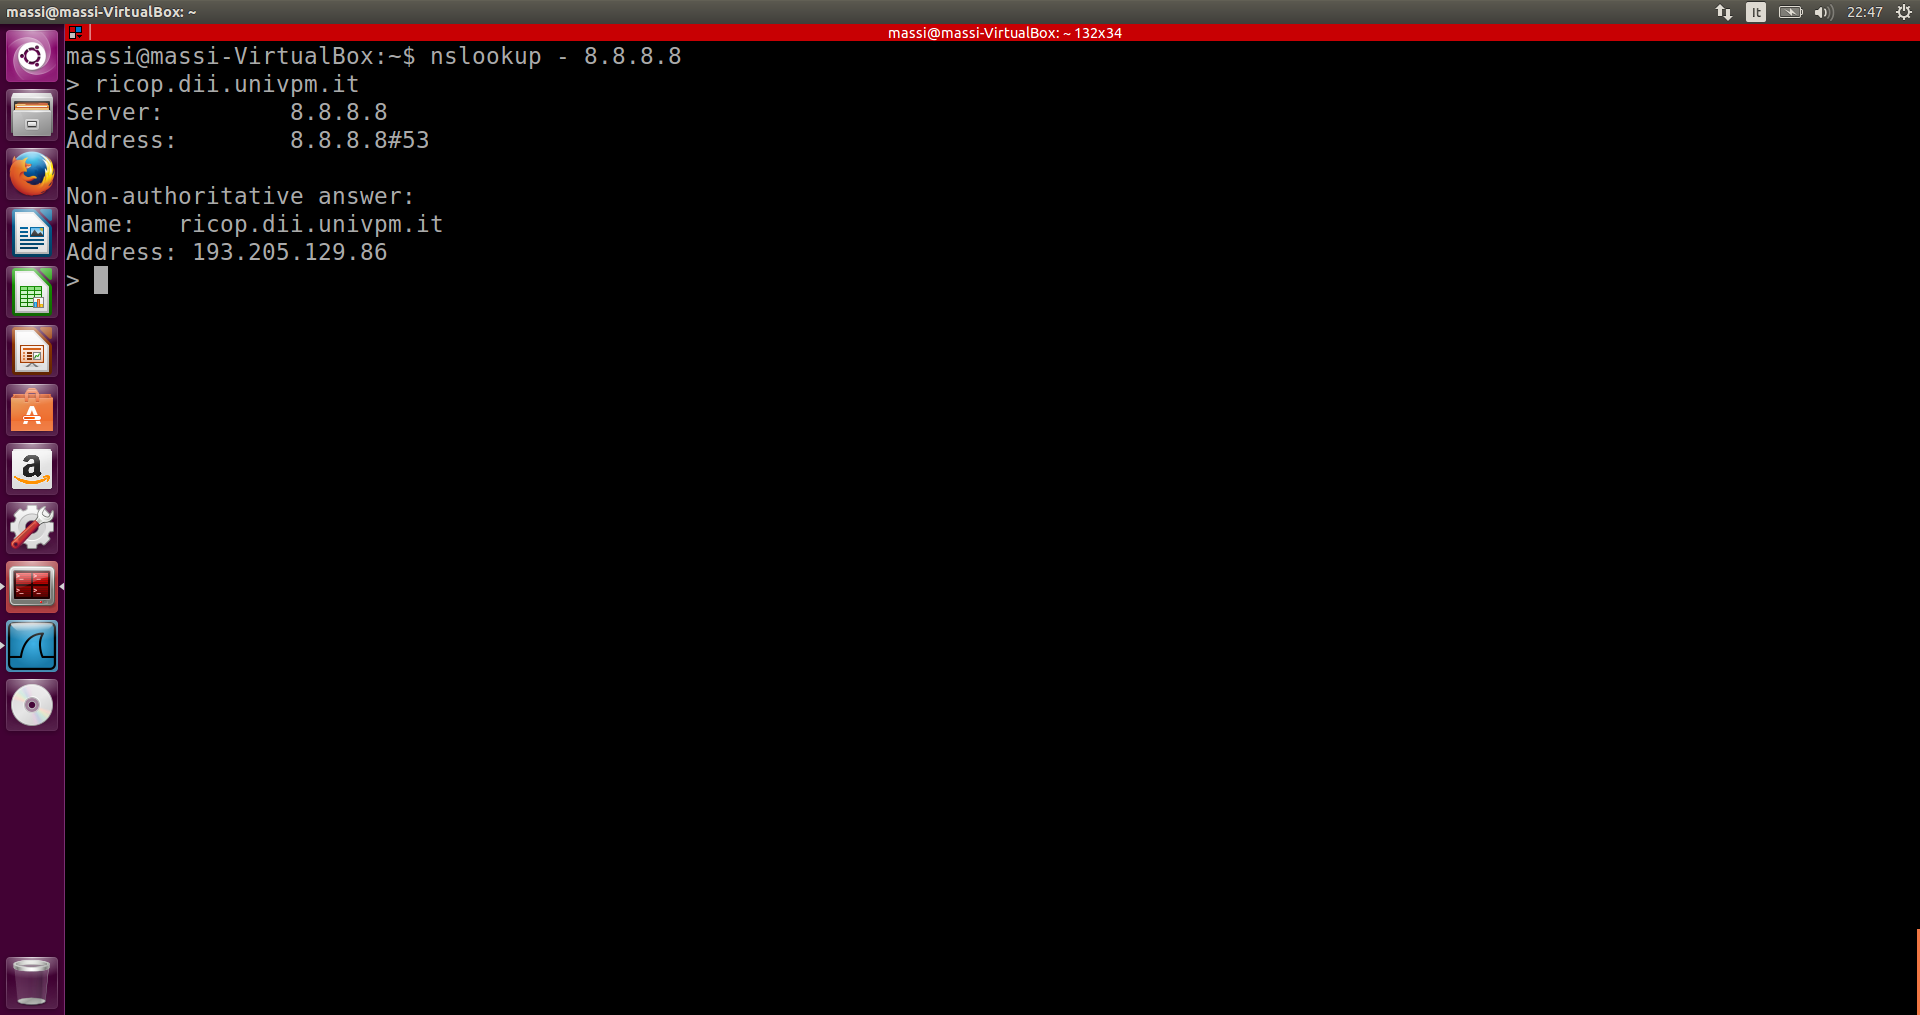
\includegraphics[width=\textwidth]{img/lab1_2}}
\only<6>{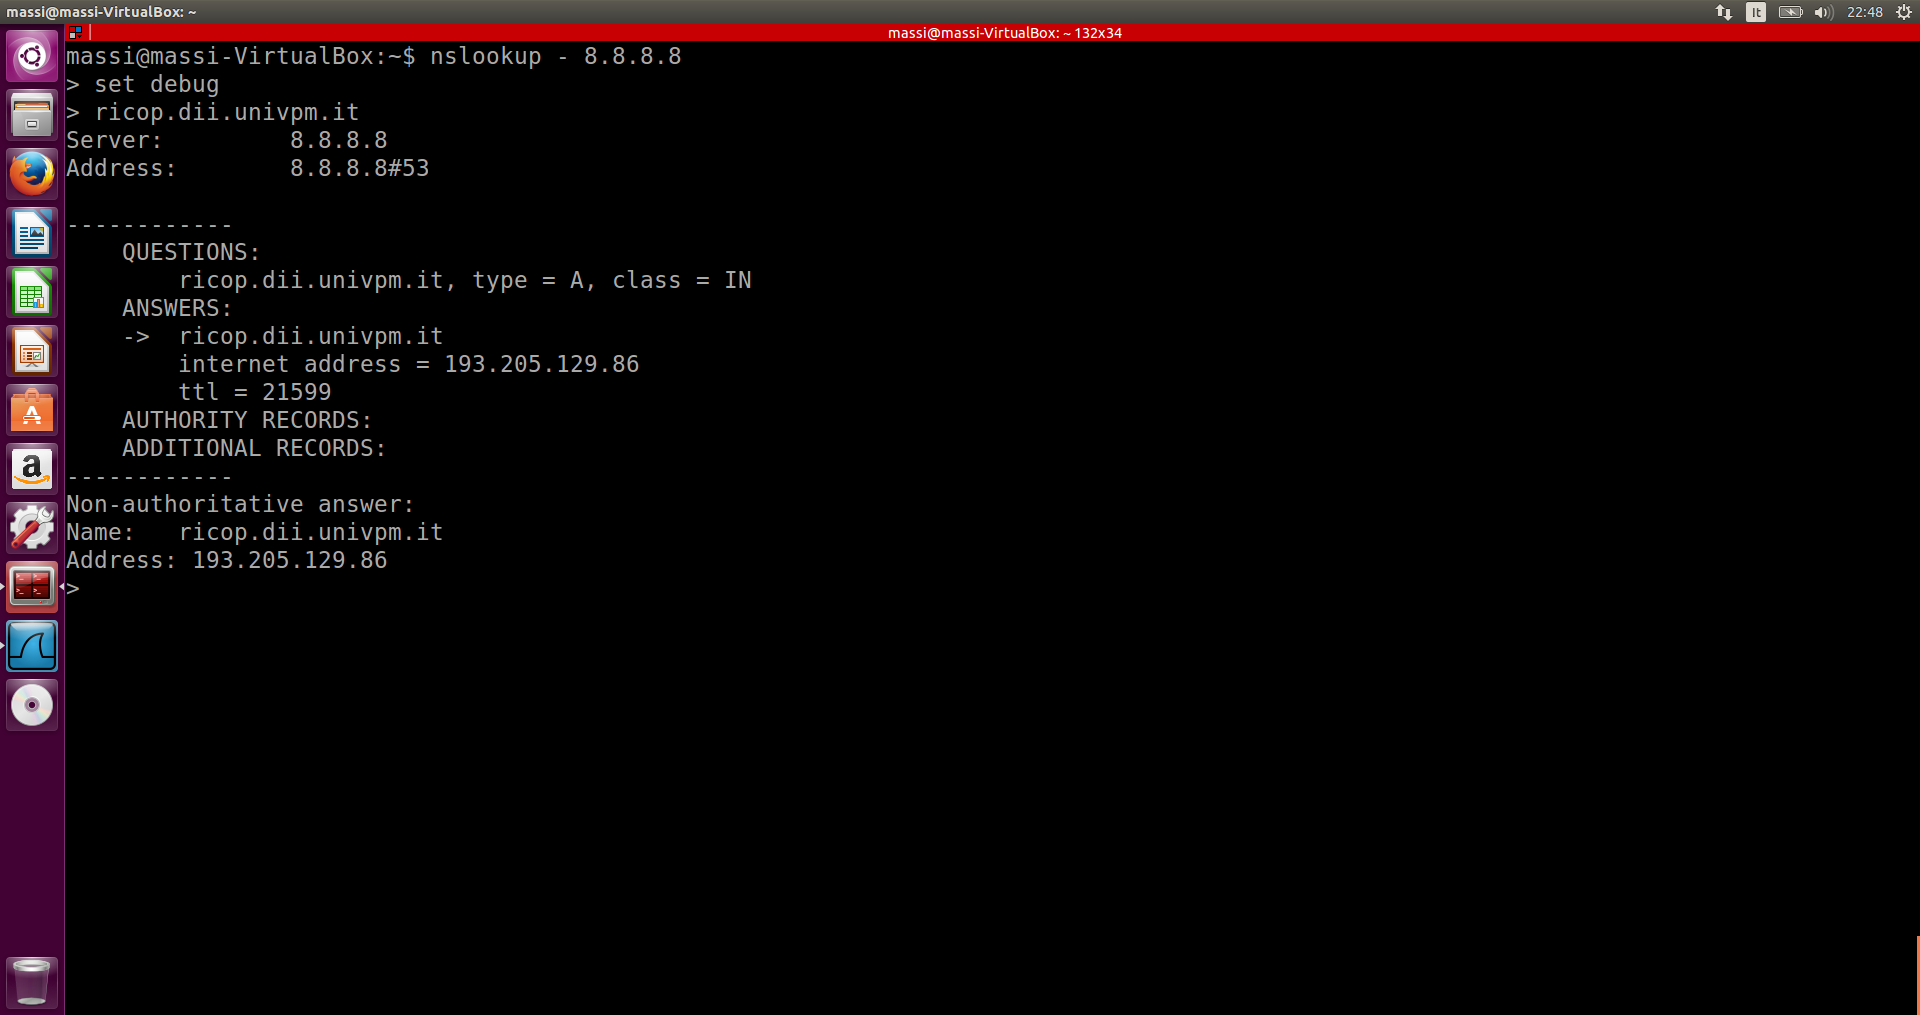
\includegraphics[width=\textwidth]{img/lab1_3}}
\only<8>{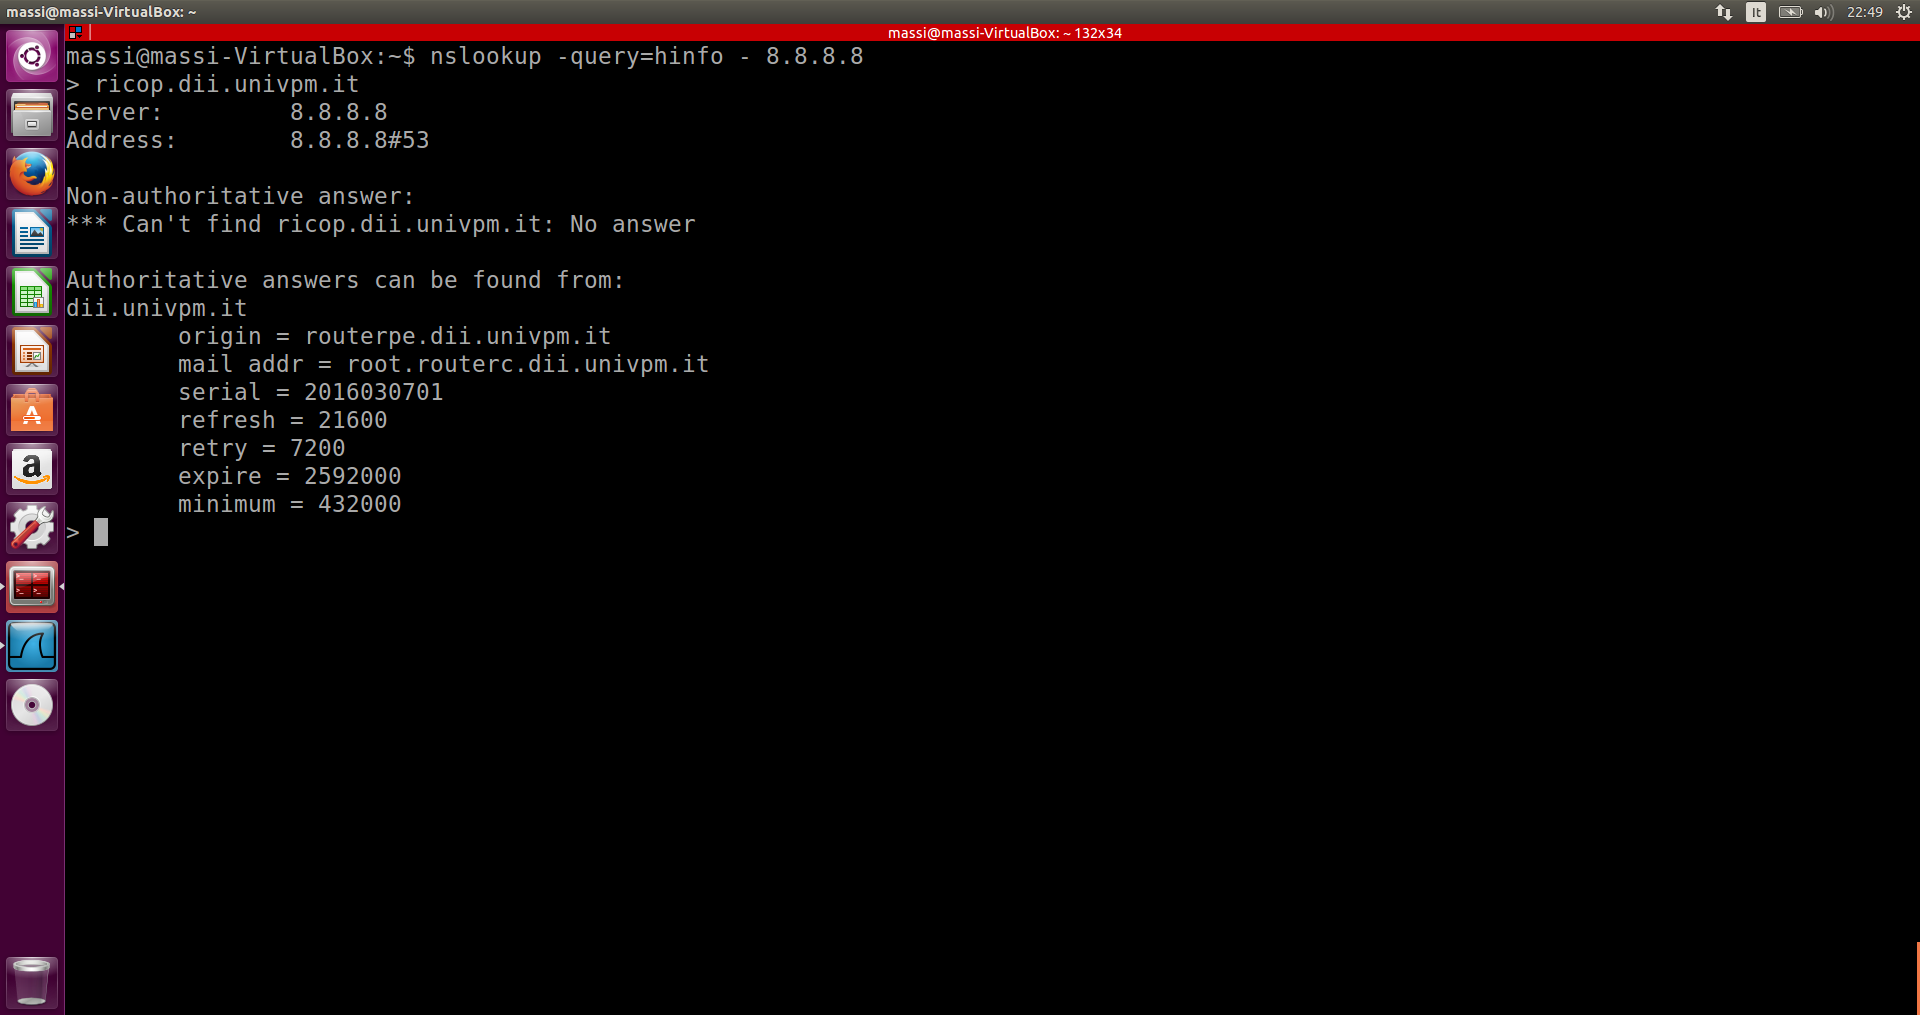
\includegraphics[width=\textwidth]{img/lab1_4}}

\end{frame}

\section[wireshark]{Analisi del protocollo DNS con \texttt{wireshark}}

\begin{frame}{Analisi del protocollo DNS}{Usare \texttt{wireshark}}

\only<1,3,5,7>{
\begin{block}{Sfide -- usare \texttt{wireshark} per visualizzare query DNS}

Wireshark lo conosciamo dai moduli precedenti (rete e trasporto).

\begin{enumerate}
	\item Come filtrare la visualizzazione dei soli pacchetti DNS? Elencare almeno due modi!
	\item \uncover<3->{Mostrare i pacchetti del protocollo DNS catturati navigando il sito wikiricop.dii.univpm.it}
	\item \uncover<5->{abilitando la visualizzazione completa del pacchetto di risposta}
	\item \uncover<7->{visualizzando le informazioni sull'host}
\end{enumerate}
\end{block}
}
%\only<2>{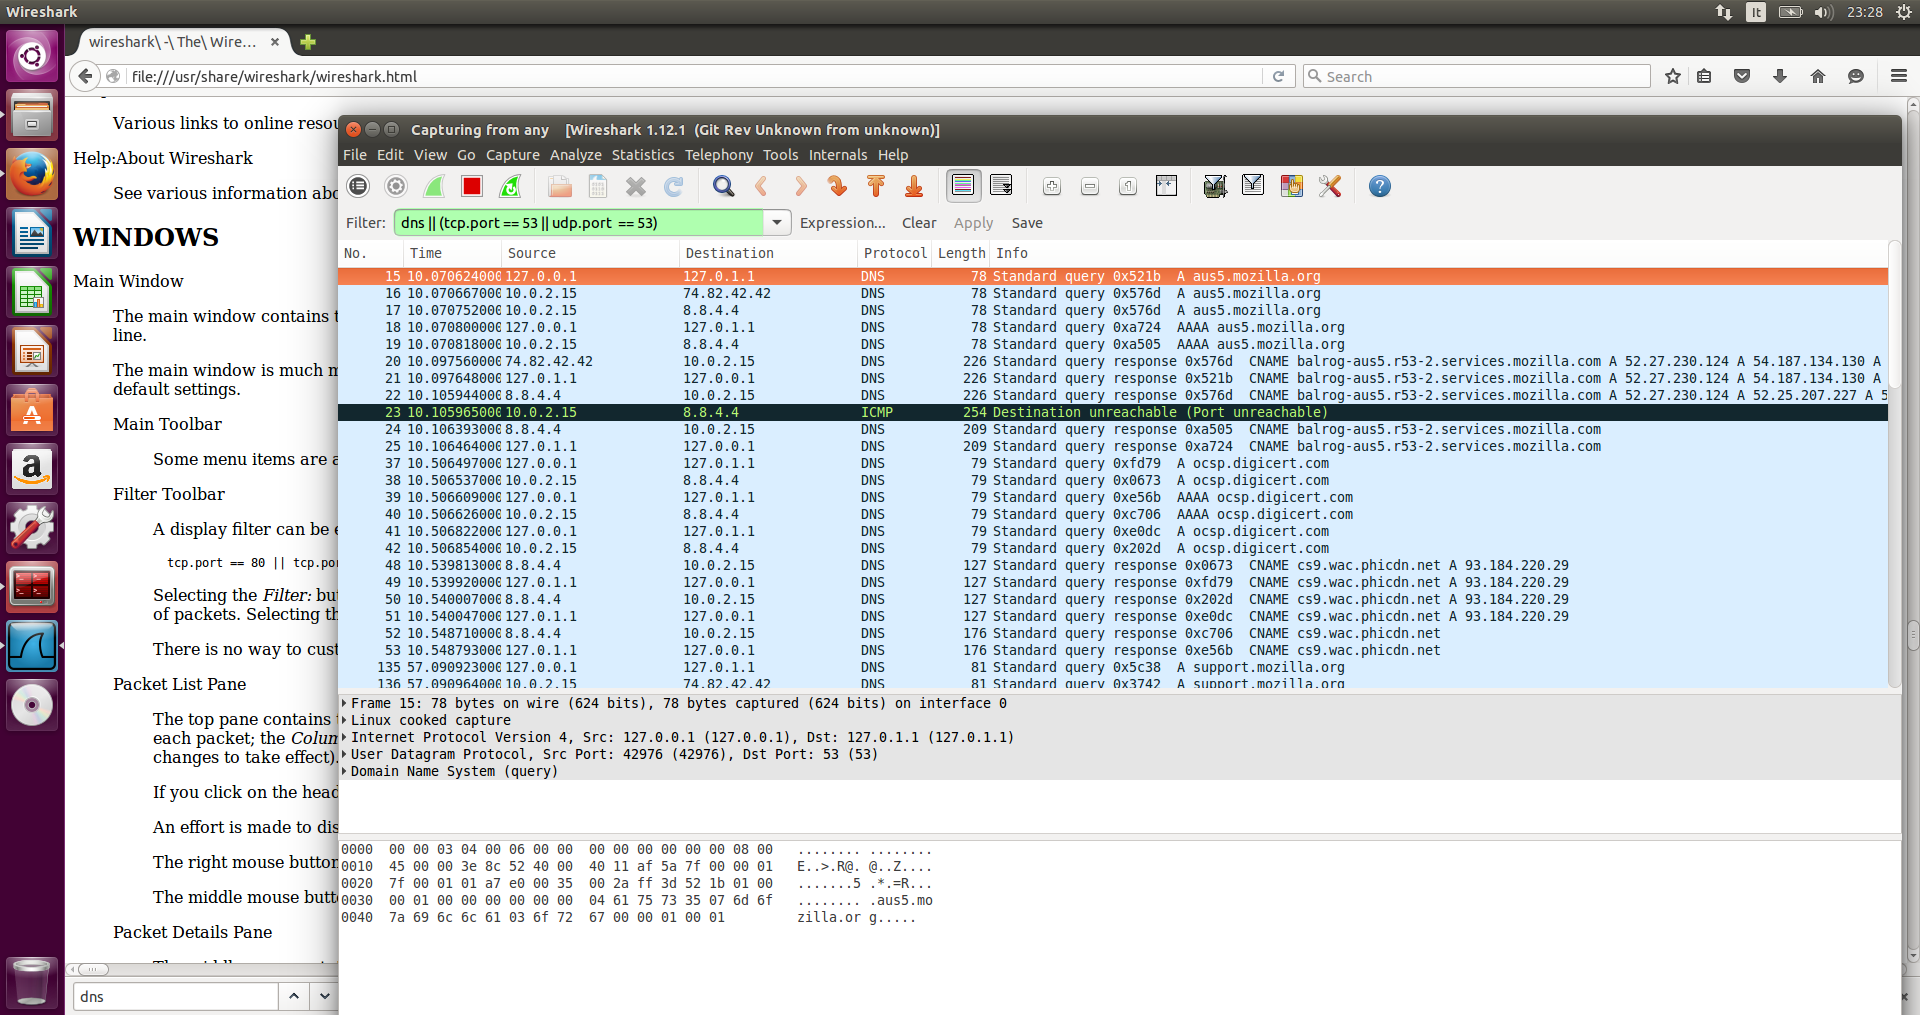
\includegraphics[width=\textwidth]{img/lab2_1}}
%\only<4>{\includegraphics[width=\textwidth]{img/lab2_2}}
%\only<6>{\includegraphics[width=\textwidth]{img/lab2_3}}
%\only<8>{\includegraphics[width=\textwidth]{img/lab2_4}}

\end{frame}

\section[Valutazione]{Valutazione}

\begin{frame}{Valutazione}{Formativa}

\end{frame}


\part[Colloquio]{Colloquio}

\begin{frame}[plain]
	
	\vfill
	
	\begin{center}
		{\Large GRAZIE PER L'ATTENZIONE!}
	\end{center}
	
	\vfill
	
\end{frame}

\end{document}

\section[Deontologia insegnamento con il software]{Deontologia professionale nell'insegnamento con il software}

\begin{frame}[allowframebreaks]{Deontologia professionale e software per la didattica}{Perch� la scuola deve usare esclusivamente software libero}
	
	
	\textbf{Le istituzioni didattiche in genere, dalla scuola materna all'universit�, hanno il dovere morale di insegnare solo il software libero.} \hyperlink{http://www.gnu.org/education/edu-schools.it.html}{\beamerbutton{Articolo di R. Stallman}}
	
	\begin{block}{Estratti I}
		Il software libero consente alle scuole di risparmiare, anche se questo � un beneficio secondario {[}\ldots{]}
		\medbreak
		La scuola ha una missione sociale: insegnare a chi studia a diventare cittadino di una societ� {[}\ldots{]} collaborativa e libera.
		\medbreak
		Al contrario, insegnare un programma non libero crea dipendenza, e questo va contro la missione sociale delle scuole: le scuole non dovrebbero mai farlo.
	\end{block}
	
	\begin{block}{Estratti II}
		\medbreak
		Il software libero consente a chi studia di poter imparare il funzionamento di un programma.
		\medbreak
		Il software libero incoraggia tutti ad imparare.
		\medbreak	
		Come si impara a scrivere codice per programmi complessi? Scrivendo tante piccole modifiche per programmi complessi esistenti. Il software libero lo permette, il software proprietario lo vieta.
		\medbreak	
		La pi� profonda motivazione in sostegno all'utilizzo del software libero nella scuola � per la formazione morale.
		\medbreak	
		Insegnare a chi studia l'uso del software libero, e a far parte della comunit� del software libero, � una lezione di educazione civica sul campo.
	\end{block}
\end{frame}

